\title{Corrections for thesis from draft v01 to draft v02}
\author{Miguel P Xochicale}
\date{ \today }

\documentclass[10pt]{article}
\usepackage[margin=0.99in]{geometry}
\usepackage{enumitem}

\begin{document}
\maketitle


\begin{abstract}
This document presents the corrections for the hand written comments 
of Chris Baber (CB) made on 21 of August 2018 for the thesis draft version 01. 
The comments of draft 01 are located in 
\emph{.../revisions/draft01-21august2018/comments/*.pdf}.
\\
\\
Additionally, I added the 3D surfaces to show the sensitivity and robustness 
of RQA metrics for different embedding parameters and recurrence thresholds.
\\
\\
Thesis draft version 02 is located at \emph{.../phd-thesis/thesis-draft02.pdf}.
\end{abstract}

%{\scriptsize
% {\tiny


%%%%%%%%%%%%%%%%%%%%%%%%%%%%%%%%%%%%%%%%%%%%%%%%%%%%%%%%%%%%%%%%%%%%%%%%%%%%%%%%
%%%%%%%%%%%%%%%%%%%%%%%%%%%%%%%%%%%%%%%%%%%%%%%%%%%%%%%%%%%%%%%%%%%%%%%%%%%%%%%%
\section{Major corrections}

\subsection{chapter 2}

\begin{enumerate}[noitemsep,topsep=0pt]
\item (p. 9) 2.2 "So - if you talk of 'error'  What is this with references to?
	What is the nonerror signal?
	How is $V_e$ actually specified/measured?
	What does $V_{nl}$ mean and how it is measured?" \\
	(p. 10) $V_e= V_{eb} +  V_{ee}+ V_{em}  $, so this say that $V_{e}$
	is made up of different components but 
	how these are measured? \\
	(p. 10) What I don't see from this is an explanation on how variability 
	is modelled or measured here. 
\begin{verbatim}
Hence, \citealt[p. 1328]{preatoni2010} concluded that the total variability 
represent the changes of contributions for $V_e$ and $V_{nl}$ 
and it is defined as $V_{tol}=V_e+V_{nl}$, where $V_{tol}$ 
"may reveal the effects of adaptation, pathologies and skills learning".
Also, \cite{preatoni2013} noted that their work only investigate error from 
biological variability (e.g. $V_{eb}$) which does not consider non-biological noise 
resulting from measuring instruments or data post-processing techniques, such 
non-biological noise has high frequency components that are usually removed.
Therefore, the work of \cite{preatoni2010} and \cite{preatoni2013} 
do not consider an overall index to quantify movement variability but 
the combination of both $V_{eb}$ and $V_{nl}$. 
With that in mind, \cite{preatoni2007} analysed the influences of 
$V_{eb}$ and $V_{nl}$ for movement repeatability by comparing 
entropy measures (e.g. ApEn and SampEn) with values of their surrogate counterparts.
\end{verbatim}
\textit{
SORTED:  Tue  4 Sep 12:02:35 BST 2018
}
\\


\item (p. 10) It would be useful to give an example here to show 
	how the parameters are measured and how they interact with each other.


\begin{verbatim}
For the experiment, \cite{muller2004} considered an skittle task, 
where participants throwing a ball with a string that swings around 
a center post with the objective of knocking down the skittle at the opposite site.
Hence, \cite{muller2004} proposed $D$ as the absolute average of distance to
the targets in $n$ trials and it is used as a measure of the collective performance 
that combines a function for movements results based on the execution vector 
with a function for the minimum distance from the target $d$.
Therefore, the overall difference in performance $D$ is decomposed
into three unequal contributions of covariation $C$, 
noise reduction $N$ and task tolerance $T$.
Considering a 2-D task spaces that spanned the release angle $\alpha$
and absolute velocity $v$, the components of contributions of
variability were calculated from five data sets ($A$, $A_0$, $A_{shift}$, $B$ and $B_0$):
(i) the component of covariation where sets $A$ and $A_0$ and $B$ and $B_0$ 
have the same means and variances,
(ii) the component of tolerance where sets $A$ and $A_{shift}$ differ only on
their location in the task space, and 
(iii) the component of noise where sets $A_{shift}$ and $B_0$ have the same
means but different variances (see Fig.6 in \cite{muller2004} for further details).
With that in mind, \cite{muller2004} conducted an experiment with forty-two participants 
for five different locations of the target skittle where for each target a participant 
performed 320 trials which is a total of 1600 trials and therefore presented 
statistical confirmation of the contributions of $T$, $N$ and $C$ using ANOVA.
\end{verbatim}
\textit{
SORTED:  Tue  4 Sep 15:02:33 BST 2018
}
\\






	
\item (p. 11) So, this discussion needs a definition (in maths) of 
	what is variability and what affects it. \\
	 (p. 11) "secondary blooming of variability" What do you mean?
\begin{verbatim}
\cite{seifert2011} investigated coordination profiles for recreational and 
competitive breaststroke swimmers and proposed an hourglass model of variability 
that illustrates the amount of variability as a function of expertise.
Hence, \citealt[p. 551]{seifert2011} stated 
recreational swimmers would show a considerable amount of intra-variability 
"as they seek an individually appropriate coordination pattern to accommodate
the novel constrains of locomotion in water", whereas experts swimmers, 
after a considerable practice,  
will still explore new environments to optimise their technique that 
create another secondary blooming of variability which is 
the result of "the environment exploration to optimise their technique 
with their individual strengths (e.g. physical, anatomical, mental, etc.)
and to gain an advantage over competitive swimmers".
To test the hourglass model of variability, 
\cite{seifert2011} considered the continuous relative phase (CRP) 
between the elbow phase angle and knee phase angle, therefore CRP 
is used as an indicator on how swimmers synchronise
arm recovery (elbow extension) and leg recovery (knee flexion).
Then, \cite{seifert2011} 
analysed inter-individual variability of swimmers with the shape of the curves 
of CRP which provide an indication of the inter-limb coordination, applied 
statistical measures such as hierarchical clustering using eleven variables of CRP 
to classify the recreational swimmers into three cluster of coordinations 
(intermediate, most-variable and in-phase)
and used Fisher information to test which CRP variables were significantly 
differientiated the clusters. With that, \cite{seifert2011} concluded that 
inter-individual coordination variability for recreational swimmers could be 
the result of (i) different state of process learning, (ii) environmental 
constraints (different perception of the aquatic resistance), or (iii) 
different perception of the task constrains (floating instead of swimming).


\end{verbatim}
\textit{
SORTED: Wed  5 Sep 10:19:27 BST 2018
}
\\



\item (p.10) So how do the two approaches (actually three: preatoni2013, muller2004 and seifer2011) differ 
	and (more importantly) What are they missing? \\
	 (p.11) good, and why would nonlinear dynamics be appropriate?
\begin{verbatim}
Generally, the previous approaches reported different models 
for movement variability which then are quantified with different tools.
For instance, \cite{hatze1986} and \cite{preatoni2010, preatoni2013} 
use entropy measures as the authors consider that the origin of the 
signals in the human body is the result of deterministic and 
stochastic processes, whereas 
\cite{muller2004} and \cite{seifert2011} reported only
statistics as a measure of magnitude that limited the evaluation of the 
whole trajectories as structures of movement variability in human body activities.
Therefore, for this thesis, it is important to note that
even with the proposed models for movement variability 
\citep{hatze1986, preatoni2010, preatoni2013, muller2004, seifert2011} 
which have been quantified it using either statistical or nonlinear tools,
little has been investigated with regards to the reliability of the nonlinear 
tools when using real data that has the property of being noisy, deterministic,
stochastic or nonstationary \citep{newell1998}.


\end{verbatim}
\textit{
SORTED: Wed  5 Sep 13:15:05 BST 2018
}
\\







\item (p. 11) This is a bad sentence that has the end repeat the start 
\begin{verbatim}
Sentence has been crossed-out
\end{verbatim}
\textit{
SORTED: Wed  5 Sep 14:00:25 BST 2018
}
\\ (p. 11) Explain the formula and why this is unacceptable. 
\begin{verbatim}
Hence, \cite{hatze1986} proposed measures of dispersion (e.g. Fourier series and 
entropy measures) to quantify the deviation of motion from a certain reference.
For which, \cite{hatze1986} pointed out that the combination 
of deviations from angular coordinates (radians) and linear coordinates (meters)
for Fourier series were unacceptable as the units are different.
Hence, \cite{hatze1986} proposed the use of entropy as a global quantifier 
for motion variability and concluded that any movement deviation on a body join 
may be the result of deterministic and stochastic causes.
\end{verbatim}
\textit{
SORTED: Wed  5 Sep 14:01:21 BST 2018
}


\item (p. 11) So entropy sounds to me like a measure of the stability 
	of a signal?
	I guess Hatze says anything that changes with time can be shown 
	to be stable?
	But you don't say why he calls it 'transentropy'
	or what is and how it is defined. 
\\ (p. 12) You don't explain the difference between stability and variability
	or what entropy is intended to measure
	\\ (p. 12)Of course it is because these are jus variations of the measure 
	why is this useful to say? 
	\\ (p. 12) So -- what do you here is name approaches without 
	(a) explain them or 
	(b) critiquing them.
	If you intent to intent to describe in more depth in a later chapter, say so.
	Also, explain why these approaches are necessary for 
	your thesis.
	
\begin{verbatim}
* "Section 2.2.1 Measures of Variability" of draft02 has been moved and 
fused with "Chapter 2: Quantifying Movement Variablity " for draft03
* Also, Chapter two answer the previous questions, specifilly the
question of 'why these approaches are neccesary for the thesis?'
\end{verbatim} 
\textit{
SORTED: Wed  5 Sep 14:15:00 BST 2018
}
\\







\item (p. 13) Why did they do this study?
	\\ (p. 13) What were the results? 
\begin{verbatim}
For example, \cite{guneysu2014} conducted experiments with children for upper 
arm rehabilitation using a play-like child robot interaction.
\cite{guneysu2014}, using a Kinect sensor to get data of join angles of 
the participants` skeleton, studied automatic evaluation of three upper body 
actions (shoulder abduction, shoulder vertical flexion and extension, 
and elbow flexion) of eight healthy children who mimicked an humanoid robot.
To evaluate motion imitation, \citealt[p. 202]{guneysu2014} considered similarity 
error using Dynamic Time Warping (DTW) that penalise large angle errors over ten 
percent in the area range of the motion type and applied recall measure 
as a representation of "how much of angular area of the baseline motion
from the humanoid robot is also covered by the child's motion".
Then, \cite{guneysu2014} presented the evaluation of five physiotherapists using 
Intraclass correlation coefficient (ICC) which a metric for reliability of 
ratings for motion types, and reported that for the first motion, which 
consists of only one join, the metric and physiotherapist evaluations 
showed hight agreements, whereas for the second and third motions, 
which motions were harder and complicated consisting of more join values, 
the evaluation between the metrics and physiotherapist presented differences.
\citealt[p. 203]{guneysu2014} stated that during the evaluation of complicated 
and harder movements, children misperceived the actions for which "therapists
compensated such misunderstanding by giving hight scores to the children
while the proposed system only considered angles".
With that, it is interesting to note that the proposed metrics of similarity 
error and recall measure with the ICC metric are not totally reliable since 
they did not model complex movements (involvement of multiple joins).
\end{verbatim}
\textit{
SORTED: Wed  5 Sep 18:30:17 BST 2018
}
\\





\item What actions? (p. 13)

\begin{verbatim}
Recently, \cite{guneysu2015} presented variation of movements from four 
physiotherapists performing five actions repeated ten times each: 
opening a door with a key, touching the opposite shoulder with hand, 
taking an object from back to neck, taking an object from the back and 
reaching an object above the head.
\end{verbatim}
\textit{
SORTED: Wed  5 Sep 20:22:05 BST 2018
}
\\



\item So -- the studies done to data have used small samples 
	and had incomplete analysis.
	What do they tell us? (p. 14)


\begin{verbatim}


For the previous works of quantifying human-robot imitation activities where 
only traditional statistics are applied,
(i) it is not only clear how \cite{gorer2013} performed the evaluation of 
synchronisation for gestures between participants and the humanoid robot 
but also the evaluation for gestures is just visual,
 whereas (ii) little has been investigated with regards to the 
differences in movement of the invited physiotherapists in the work of
\cite{guneysu2014} and  \cite{guneysu2015}.
Therefore, it is noted that applying nonlinear analyses instead of 
traditional statistics in the context of human-robot interaction 
might provide a better quantification and understanding human movement.



\end{verbatim}
\textit{
SORTED: Thu  6 Sep 11:16:10 BST 2018
}
\\




\item Explain in more detail (p. 14)

\begin{verbatim}

Two participant's movement positions were presented with twelve trajectories each
(four dance activities times three trials) of z and x directions obtained with 
a Kinect sensor.

\end{verbatim}
\textit{
SORTED: Thu  6 Sep 11:31:34 BST 2018
}
\\



\item It would be good to know more about the data (p. 14) \\
	 So -- how will your thesis fill these gaps? (p. 14)

\begin{verbatim}

The following section 
\section{Gaps in the study of Movement Variability in the 
	context of Human-Humanoid Interaction}
was fused with 
\section{Movement Variability in the context of Human-Humanoid Interaction}
in which works of 
has been reviewed  and then pointed out
how their limitations can be tackled in this thesis.

\end{verbatim}
\textit{
SORTED: Fri  7 Sep 13:06:10 BST 2018
}




\end{enumerate}




\subsection{chapter 4}


\begin{enumerate}[noitemsep,topsep=0pt]
\item explain what is meant by an embedding parameter (p. 21)

\begin{verbatim}
The method of state space reconstruction is based on uniform time-delay 
embedding which is a simple matrix implementation considering the embedding 
parameters ($m$ and $\tau$), therefore, matrix represents the reconstruction
of an unknown $d-$dimensional manifold $M$ from a scalar 
time series (e.g. one-dimensional time series in $\mathbb{R}$).
\end{verbatim}
\textit{
SORTED: Mon 10 Sep 10:04:07 BST 2018
}



\item you haven't explained 'attractor' or how this is folded
	(in a manifold) (p. 25)

\begin{verbatim}

Then, if $\Phi$ is an embedding of an attractor (i.e. evolving 
trajectories) in the reconstructed state space, a composition of functions 
represented with $F^t$ is induced on the reconstructed state space:

.
.
.


attractor (i.e. evolving trajectories in a state space) 
\end{verbatim}
\textit{
SORTED: Mon 10 Sep 14:08:24 BST 2018
}
\\




\item not sure I see this at $m \geq 5$ don't these equal to one. (p.28)

\begin{verbatim}

Althought the $E_2(m)$ values for the chaotic time series tend to be closer to
one as $m$ increses, these are different to one (Fig~\ref{fig:e1e2}C), 
for which, it can be concluded that the chaotic time series comes 
from a chaotic deterministic signal.
...
Then, contrary to the $E_2(m)$ values for a chaotic 
Lorenz time series, all values of $E_2(m)$ for a noise time series are 
approximately equal to one (Figure~\ref{fig:e1e2}D). 


\end{verbatim}
\textit{
SORTED: Mon 10 Sep 15:39:12 BST 2018
}
\\



 
\item report in the last chapter (p. 29) 
\begin{verbatim}
Negatives of False Nearest Neighbor were moved to future work section
\end{verbatim}
\textit{
SORTED: Mon 10 Sep 15:45:54 BST 2018
}
\\



\item give numbers to define these (p. 31)
\begin{verbatim}
For small $\tau$ ($\tau < 3$), AMI will be large ( $I(\tau)>6$)and as 
$m$ increase AMI will then decrease rapidly. 
\end{verbatim}
\textit{
SORTED: Mon 10 Sep 16:21:32 BST 2018
}
\\




\item (p. 28) so -- how does this compare to page 28? \\
	(p. 32) so, which one do you use and why? 


\begin{verbatim}
\subsection{Minimum embedding parameters}
The method to select minimum embedding parameters ($m_0$ and $\tau_0$) 
for this thesis is firstly to compute $m_0$ with FNN algorithm 
(considering a threshold of 0.05 for $E_1(m)$ values), secondly
to compute $\tau_0$ with AMI which does not need any extra parameters.
Hence, from the previous example of the chaotic deterministic 
Lorenz system, Fig \ref{fig:e1e2}(A) is used to determine the minimum 
dimension embedding with a value of seventeen ($m_0 =6$) and 
Fig \ref{fig:amis}(A) is used to determine the minimum delay embedding 
with a value of seventeen ($\tau_0 =17$). 
Therefore with the selection of the minimum embedding parameters, the 
reconstructed attractor is created in order to ensure with $\tau_0$ the 
maximum independence between $x(t)$ and $x(t+\tau_0)$ and with $m_0$ 
allowing the trajectories in the reconstructed state space to be unfolded.


\end{verbatim}
\textit{
SORTED: Tue 11 Sep 11:01:20 BST 2018
}
\\





\item (p. 32) so -- do you need this section?
\begin{verbatim}
section: Other methodologies for state space reconstruction
has been moved to future work in chapter 7.
\end{verbatim}
\textit{
SORTED: Tue 11 Sep 11:03:47 BST 2018
}
\\




\item You haven't defined this or explained it (p. 38)
\begin{verbatim}
Lyapunove exponents are briefly explained in 
{chapter2/chapter} %Quantifying Movement Variability
\end{verbatim}
\textit{
SORTED: 
Tue 11 Sep 11:07:05 BST 2018
}
\\






\item (p. 41) I think that the chapter shows quite well 
	that you understand the various methods and can explain them.
	Why you don't do is explain why you will use these particular methods.	
	\\ - Why are they appropriate to the type of data you intent to collect, 
	\\ - the type of variability you expect to see, 
	\\ - or the type of analysis you intent to make?
	You should explain your choice of method to the reader.




\begin{verbatim}
Therefore, considering 
(i) the strengthens and weaknesses of different nonlinear tools when 
using real-world data which is nonstationarity, noisy and has different 
sampling rate and length (Section \ref{nonlieaRealdata}),
(ii) not only the model of \cite{stergiou2006} where complexity and 
predictability variables can characterise movement variability but also
the dependency of the task dynamics 
\citep{vaillancourt2002, vaillancourt2003} 
(Section \ref{what_to_measure_with_MV}), and 
(iii) the selection and application the right tools in order to quantify MV
(Section \ref{which_NT_are_appropriate_to_measure_MV}).
We therefore explore, in this thesis, the sensitivity and robustness of 
the window size of time series, embedding parameters for RSS with UTDE 
and recurrence threshold for RP and RQA in order to gain a 
better insight into the underlying time series collected from inertial 
sensors in the context of human-humanoid imitation activities.
\end{verbatim}
\textit{
SORTED: Tue 11 Sep 13:29:38 BST 2018
}
\\



	
\end{enumerate}









\subsection{chapter 5}


\begin{enumerate}[noitemsep,topsep=0pt]
\item This should be written as an Experiment Method Chapter: \\
	1. Aims \\
	2. Participants \\
	3. Equipment \\
	4. Procedures / ethics \\
	5. Data preparation \\
		each section should have detail
		to allow the experiment to be replicated 
		\\
	I would expect this chapter to be 10 pages long (at least)


\begin{verbatim}

Updated Outline for chapter

2 Experiments
2.1 Aims 
2.2 Participants 
2.2.1 Human-Image Imitation Activities 
2.2.2 Human-Humanoid Imitation Activities
2.3 Equipment
2.4 Ethics 
2.5 Experiments 
2.5.1 Human-Image Imitation Activities 
2.5.2 Human-Humanoid Imitation Activities 
2.6 Preparation of time series 
2.6.1 Raw time-series 
2.6.2 Postprocessing time-series 
2.6.3 Normalization of time-series 
2.6.4 Smoothing time-series 
2.6.5 Window size of time-series 

\end{verbatim}
\textit{
SORTED: 
Wed 12 Sep 14:31:29 BST 2018
}
\\




\item 5.1, 5.2 and 5.3 (each of these) could be illustrated from the images
	from the images from your instructions (p. 45)


\begin{verbatim}

%%---------------------------------(FIGURE)-------------------------------------
\begin{figure}
  \centering
  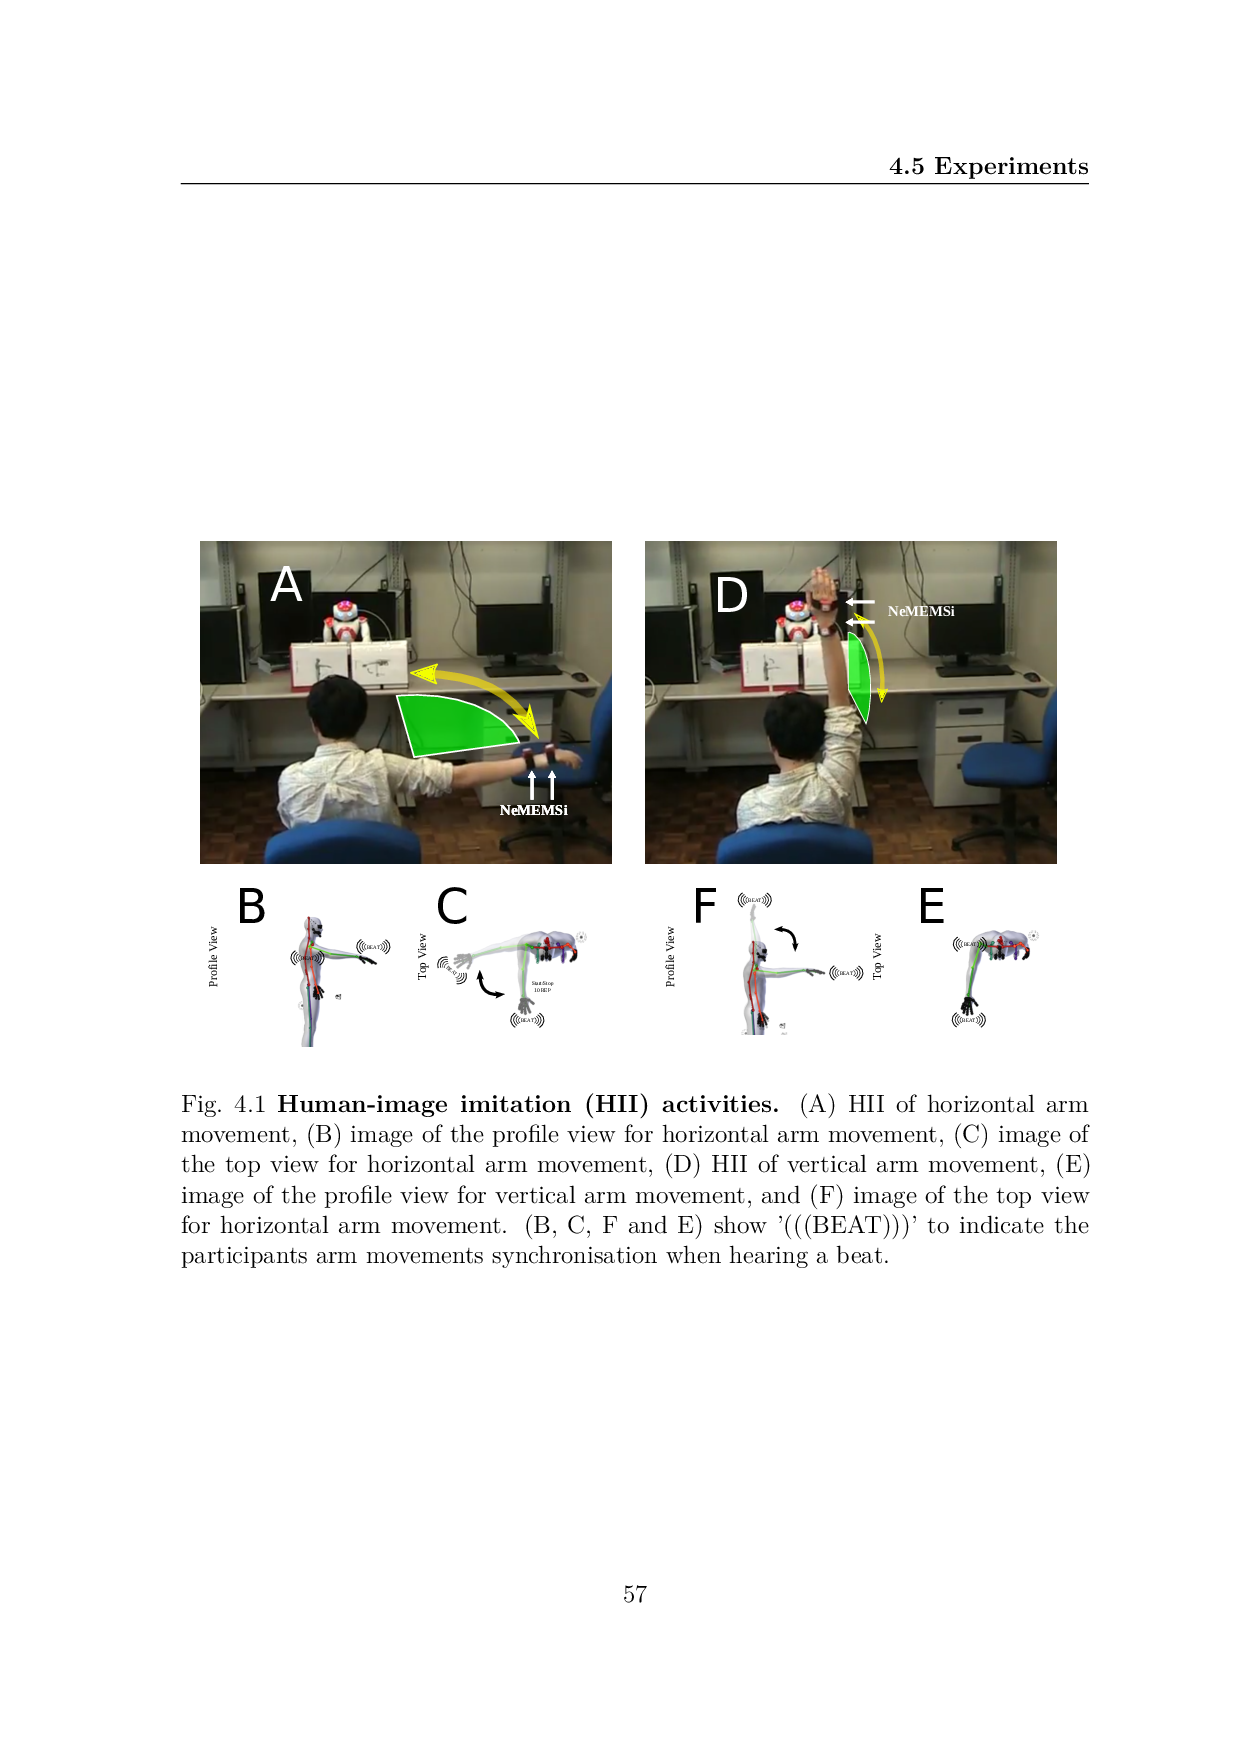
\includegraphics[width=1.0\textwidth]{hii}
    \caption{
	{\bf Human-image imitation (HII) activities.} 
		%Human-image imitation (HHI) activities for 
		(A) HII of horizontal arm movement, 
		(B) image of the profile view for horizontal arm movement,
		(C) image of the top view for horizontal arm movement,
		(D) HII of vertical arm movement, 
		(E) image of the profile view for vertical arm movement, and
		(F) image of the top view for horizontal arm movement.
		(B, C, F and E) show '(((BEAT)))' to indicate the participants
		arm movements synchronisation when hearing a beat.
        }
    \label{fig:hii}
\end{figure}
%%---------------------------------(FIGURE)------------------------------------

\end{verbatim}
\textit{
SORTED: 
Wed 12 Sep 14:26:18 BST 2018
}
\\






\item (p. 45) Ethics -- you should say that the design of the experiment 
	adhered to UoB regulations. 
	Data were anonymised and stored only on your computer.
	Participants provided informed consent and were free to 
	withdraw from the study	(p. 45).


\begin{verbatim}

\section{Ethics}
For the experiments of this thesis conducted in November 2016, 
participants confirmed reading and understanding the participant information 
sheet for the experiments and were able to withdraw from the experiment 
at any time without giving any reason.
The design of the experiments is adhered to University of Birmingham 
regulations and data were anonymised and stored only a personal 
computer in accordance with the Data Protection Act 1998.
For further information about the ethics, online participation 
information sheets and experiment check list, refer to 
Appendix \ref{appendix:c}.

\end{verbatim}
\textit{
SORTED: 
Wed 12 Sep 14:27:53 BST 2018
}
\\





	
\end{enumerate}













\subsection{chapter 7}

\begin{enumerate}[noitemsep,topsep=0pt]
\item move the underlined section to previous chapter!

\begin{verbatim}
\section{Human-Humanoid Imitation Experiment} % \label{sec:experiment}
were moved and polished to previous chapter (Time series dataset)
\end{verbatim}
\textit{
SORTED: 
Tue 11 Sep 13:51:14 BST 2018
}
\\




\item (p. 49) "results from three participants". 
	I don't see that these are 'space' problems for a thesis
	-- perhaps choice of three to make comparison easier?
	Other data in Appendix X. (p. 55)

\begin{verbatim}

To make comparison easier, we only present 10-sec (500 samples) window length 
time series for three participants (p01, p01 and p03) performing horizontal 
arm movements (axis GyroZ) and  vertical arm movements (axis GyroY) 
(Figs \ref{fig:tsH} and \ref{fig:tsV}), other data is presented in 
Appendix \ref{appendix:d}.

\end{verbatim}
\textit{
SORTED: 
Wed 12 Sep 18:01:01 BST 2018
}
\\




\item (p. 57) So -- rather than 'individual' you use 'sample' 
	$m+1$ 
	but this is a new step that you haven't explained previously.
	Be a good idea to anticipate this in your Metrics chapter
	or you move your points on page 59/60 earlier. 


\begin{verbatim}

\subsection{Overall minimum embedding parameters} \label{sec:overall_minMT}
We use sample mean for an overall value of embedding minimum embedding 
parameters ($\overline{m}_0$, $\overline{\tau}_0$) in which minimum values 
($m_{0_i}$, $\tau_{0_i}$) are averaged over $N$ which is the total number 
of minimum embedding values:
\begin{equation}
	\overline{m}_0= \frac{1}{N} \sum^{N}_{i = 1} m_{0_i},
\end{equation}
\begin{equation}
	\overline{\tau}_0= \frac{1}{N} \sum^{N}_{i = 1} \tau_{0_i}.
\end{equation}


\end{verbatim}
\textit{
SORTED: Thu 13 Sep 12:40:41 BST 2018
}
\\






\item (p. 58)  Fig 7.6 Should be bigger and clearer
	\\  (p. 59) Figs. 7.7 and 7.8 Should be bigger and clearer

\begin{verbatim}
Figs were changed to a bigger size and look clearer.
\end{verbatim}
\textit{
SORTED: 
Wed 12 Sep 20:18:51 BST 2018
}
\\





\item (p. 59) This sentence doesn't make sense


\begin{verbatim}

Although the implementation of Uniform Time-Delay Embedding matrix (UTDE) 
is simple, the main challenge in this regard is to select embedding parameters 
to reconstruct the state spaces for each time series, considering that time 
series are unique in terms of its structure (modulation of amplitude, 
frequency and phase) \citep{ frank2010, sama2013, bradley2015}.
With that in mind, the problem is not to compute individual embedding parameters 
for each of the time series but to deal with a selecting of two parameters 
that can represent all the time series. 

\end{verbatim}
\textit{
SORTED: 
Thu 13 Sep 13:47:20 BST 2018
}
\\





\item (p. 60) You should point some examples out to the reader -- 

\begin{verbatim}

(Section \ref{sec:rsswithUTDE}) in Chapter 3 were created 
to give more details about the RSSwUTDE and examples

\end{verbatim}
\textit{
SORTED: 
Thu 13 Sep 19:44:32 BST 2018
}
\\


	what are the figures 7.9 and 7.10 showing?
	What are the relevant or important things to notice?
	I think there is at least another page of explanation 
	provide here.


\begin{verbatim}

The RSSs for horizontal normal and faster from the human sensors (HS01)
are slightly smoothed as the time-series smoothness increase
Figs~\ref{fig:rss_aHw10}(A,C). Similarly, the smoothness of RSSs 
for robot sensor (RS01) is smoothed as the time series smoothness increase.
Although the frequency of the movement increase from normal to faster velocity, 
the RSSs in Figs~\ref{fig:rss_aHw10}(B)
show highers osciallations specially for a maximum values of smoothnes,
while the RSS for HF in Figs~\ref{fig:rss_aHw10}(D) show a lower and smothed
osicallations as the smoothenss increase.


Although time series for vertical movements are less noisy and well structured
(Figs \ref{fig:tsV}), the RSSs (Figs \ref{fig:rss_aVw10}) seems to be less 
organised, specially for Fig \ref{fig:rss_aVw10}(A,C), while time series 
for vertical faster movements (VF) having more periods (Figs \ref{fig:tsV})
create RSS with well defined patters (\ref{fig:rss_aVw10}(C,D)).
It is important to note that smoothness of time series creates also an effect
on smoothness in the trajectories of the RSS being the RS01 more organised
and more persistent while trajectories for HS01 are more changeable.




\end{verbatim}
\textit{
SORTED: 
Fri 14 Sep 06:32:08 BST 2018
}
\\





\item (p. 61) Figs 7.9 should be bigger and clearer
	\\ (p. 62) Figs 7.10 should be bigger and clearer


\begin{verbatim}

Therefore, considering time series for participant 01 
(Figs \ref{fig:tsH}, \ref{fig:tsV}) the reconstructed state spaces
for horizontal arm movements (Figs~\ref{fig:rss_aHw10}) and
 vertical arm movements  (Figs~\ref{fig:rss_aVw10}) 
are computed with $\overline{m_0}=6$ and $\overline{\tau_0}=8$ 
(Section \ref{sec:rsswithUTDE}).

\end{verbatim}
\textit{
SORTED: 
Thu 13 Sep 19:46:56 BST 2018
}
\\













\item (p. 62) Again -- explain this figures and point out the important 
	relevant features.
	Don't assume the reader will see everything that you do.


\begin{verbatim}

Generally, the increase of smoothness in time series results in ticker 
and more well defined diagonal lines in the RPs 
Regarding the low and hight frequencies in the time series due to the 
changes in velocities of the movements, RPs patterns
show both an increase of diagonal lines and a decrease of its thickness.
Although, RPs patterns show consistency with the movements type and velocities,
it can be noticed that RPs for HS01 are not entirely well defined
while RPs for RS01 shown a more consistent pattern
(Fig~\ref{fig:rp_aV}, \ref{fig:rp_aH}). 

\end{verbatim}
\textit{
SORTED: 
Fri 14 Sep 11:19:36 BST 2018
}
\\




\item (p. 63) Figs 7.11 should be bigger and clearer


\begin{verbatim}
Amended figure size and also added a better descrition for the caption
\end{verbatim}
\textit{
SORTED: 
Fri 14 Sep 11:18:49 BST 2018
}
\\






\item (p. 63) "HS01" Is this from one person? Explain what
	HS01 means, and why use these data.

\item (p. 65) Would you expect them to change?

\item (p. 68) This belongs to earlier in the metrics review chapter

\item (p. 70) Every figure should have at least one paragraph of explanation
	to point out key features 

\item I can see you have produced results 
	but it is not obvious how these are meant to be interpreted.
	You need more explanation of the important and relevant elements
	of each figure.
	You need to say whether the results are expected and
	whether different methods agree or contradict each other. \\
	I am also worried that not including any of  your other data
	means you risk the thesis looking like a single study 
	MSc by Research rather than a PhD.


\end{enumerate}



\subsection{chapter 8}

\begin{enumerate}[noitemsep,topsep=0pt]

\item What were the research questions? \\
	How were these answered?\\
	How does your work extend and advance the field?\\
	(p. 73)

\end{enumerate}







\section{Minor Corrections}

%%%%%%%%%%%%%%%%%%%%%%%%%%%%%%%%%%%%%%%%%%%%%%%%%%%%%%%%%%%%%%%%%%%%%%%%%%%%%%%%
%%%%%%%%%%%%%%%%%%%%%%%%%%%%%%%%%%%%%%%%%%%%%%%%%%%%%%%%%%%%%%%%%%%%%%%%%%%%%%%%
\subsection{title}

\begin{itemize}[noitemsep,topsep=0pt]
\item Changing title\\

\textit{
\title{Nonlinear Time-series Analysis for Movement Variability in 
Human-humanoid Interaction} }


\textit{
\\
SORTED: Mon  3 Sep 13:05:34 BST 2018 
}
\end{itemize}



%%%%%%%%%%%%%%%%%%%%%%%%%%%%%%%%%%%%%%%%%%%%%%%%%%%%%%%%%%%%%%%%%%%%%%%%%%%%%%%%
%%%%%%%%%%%%%%%%%%%%%%%%%%%%%%%%%%%%%%%%%%%%%%%%%%%%%%%%%%%%%%%%%%%%%%%%%%%%%%%%
\subsection{toc}

\begin{itemize}[noitemsep,topsep=0pt]
\item Comments about the use of English language!

\textit{
\\
SORTED:  Mon  3 Sep 13:19:58 BST 2018
}

\end{itemize}

%%%%%%%%%%%%%%%%%%%%%%%%%%%%%%%%%%%%%%%%%%%%%%%%%%%%%%%%%%%%%%%%%%%%%%%%%%%%%%%%
%%%%%%%%%%%%%%%%%%%%%%%%%%%%%%%%%%%%%%%%%%%%%%%%%%%%%%%%%%%%%%%%%%%%%%%%%%%%%%%%
\subsection{chapter 1}

\begin{itemize}[noitemsep,topsep=0pt]
\item Comments about the improvement of use of English language. \\

\item References need to be in Harvard style. 

\textit{
\\
SORTED:  Mon  3 Sep 15:00:10 BST 2018
}



\end{itemize}




\subsection{chapter 2}

\begin{itemize}[noitemsep,topsep=0pt]
\item All References need to be in Harvard style.
 
\item 2.1 comments are essentially about improvement of use of English.

\item when quoting someone, use page number.

\item modify title of 2.4 which reads like:
	Gaps in the study of movement variability in the context of 
	human-humanoid interaction (p. 14)


\textit{
\\
SORTED:  Mon  3 Sep 23:24:44 BST 2018
}



\end{itemize}

\subsection{chapter 3}

\begin{itemize}[noitemsep,topsep=0pt]


\item Corrections with the use of English language

\item 'Spell out acronyms in headings'
	e.g. RSS, RP and RQA

\begin{verbatim}
Spelling errors, corrections with the use of English and
well defined references were improved
\end{verbatim}
\textit{
SORTED: Mon 10 Sep 14:00:19 BST 2018
}
\\




\end{itemize}

\subsection{chapter 4}

\begin{itemize}[noitemsep,topsep=0pt]
\item Corrections with the use of English language
	and citations.
\end{itemize}






\section{MX corrections}

\subsection{chapter 1}





\subsection{chapter 2}


\begin{enumerate}

\item Solve the following questions for the fusion of 
	"Section 2.2.1 Measures of Variability" of draft02 
	with "Chapter 2: Quantifying Movement Variablity " for draft03,
	mainly answer 'why these approaches are neccesary for the thesis?':
	\\ (*) So entropy sounds to me like a measure of the stability 
	of a signal?
	I guess Hatze says anything that changes with time can be shown 
	to be stable?
	But you don't say why he calls it 'transentropy'
	or what is and how it is defined. 
	\\ (*) You don't explain the difference between stability and variability
	or what entropy is intended to measure
	\\ (*) Of course it is because these are jus variations of the measure 
	why is this useful to say? 
	\\ (*) So -- what do you here is name approaches without 
	(a) explain them or 
	(b) critiquing them.
	If you intent to intent to describe in more depth in a later chapter, say so.
	Also, explain why these approaches are necessary for 
	your thesis.

\begin{verbatim}
Previous questions are anwered with the updated chapter 2: 
"Quantifying movement variability"
\end{verbatim}
\textit{
SORTED: Sun  9 Sep 23:44:20 BST 2018
}

	
\end{enumerate}


\end{document}

